\section{Обробка слайдів}
\vspace{-\baselineskip}
\subsection{Порівняння слайдів}

Після видалення викладача та суміщення кадрів ми створюємо слайди у вигляді
коротких нотаток лекції. Ми по черзі беремо пари кадрів панорами, які
необов'язково є сусідніми~---~для збільшення чутливості алгоритму створення нових
слайдів можна використовувати кадри, різниця між індексами яких є більшою, бо
змін на дошці між сусідніми кадрами може не бути.

Ми використовуємо оператор Лапласа \cite{website:scikit-image} для знаходження перепадів
яскравості і зменшення рівня шуму. У наших експериментах саме цей
оператор надав кращі результати, ніж інші диференціальні оператори

\begin{equation*}
  L(x,y) = \nabla^{2}f(x,y) = \frac{\partial^{2}f(x,y)}{\partial x^{2}} + \frac{\partial^{2}f(x,y)}{\partial y^{2}}.
\end{equation*}

Для одержання маски всіх написів на дошці застосовуємо метод бінаризації
Оцу \cite{website:scikit-image}. Це швидкий алгоритм, який на наш погляд дає прийнятну
якість бінаризації для створення слайдів (рис. \ref{fig:binarized_slide_example}).


Не кожна панорама є новим слайдом. Коли зміни на дошці невеликі
(наприклад, лектор дописав формулу), треба лише оновити існуючий слайд.
Якщо ж зміни значні (наприклад, лектор стер попередні записи), треба
створити новий слайд і працювати з ним. Щоб мінімізувати недоліки маски
та отримувати слайди з новою інформацією на дошці, ми виділяємо нові
написи за допомогою оператора Лапласа.
\begin{figure}[H]
  \centering
  \subfloat[Кадр з відео]{
    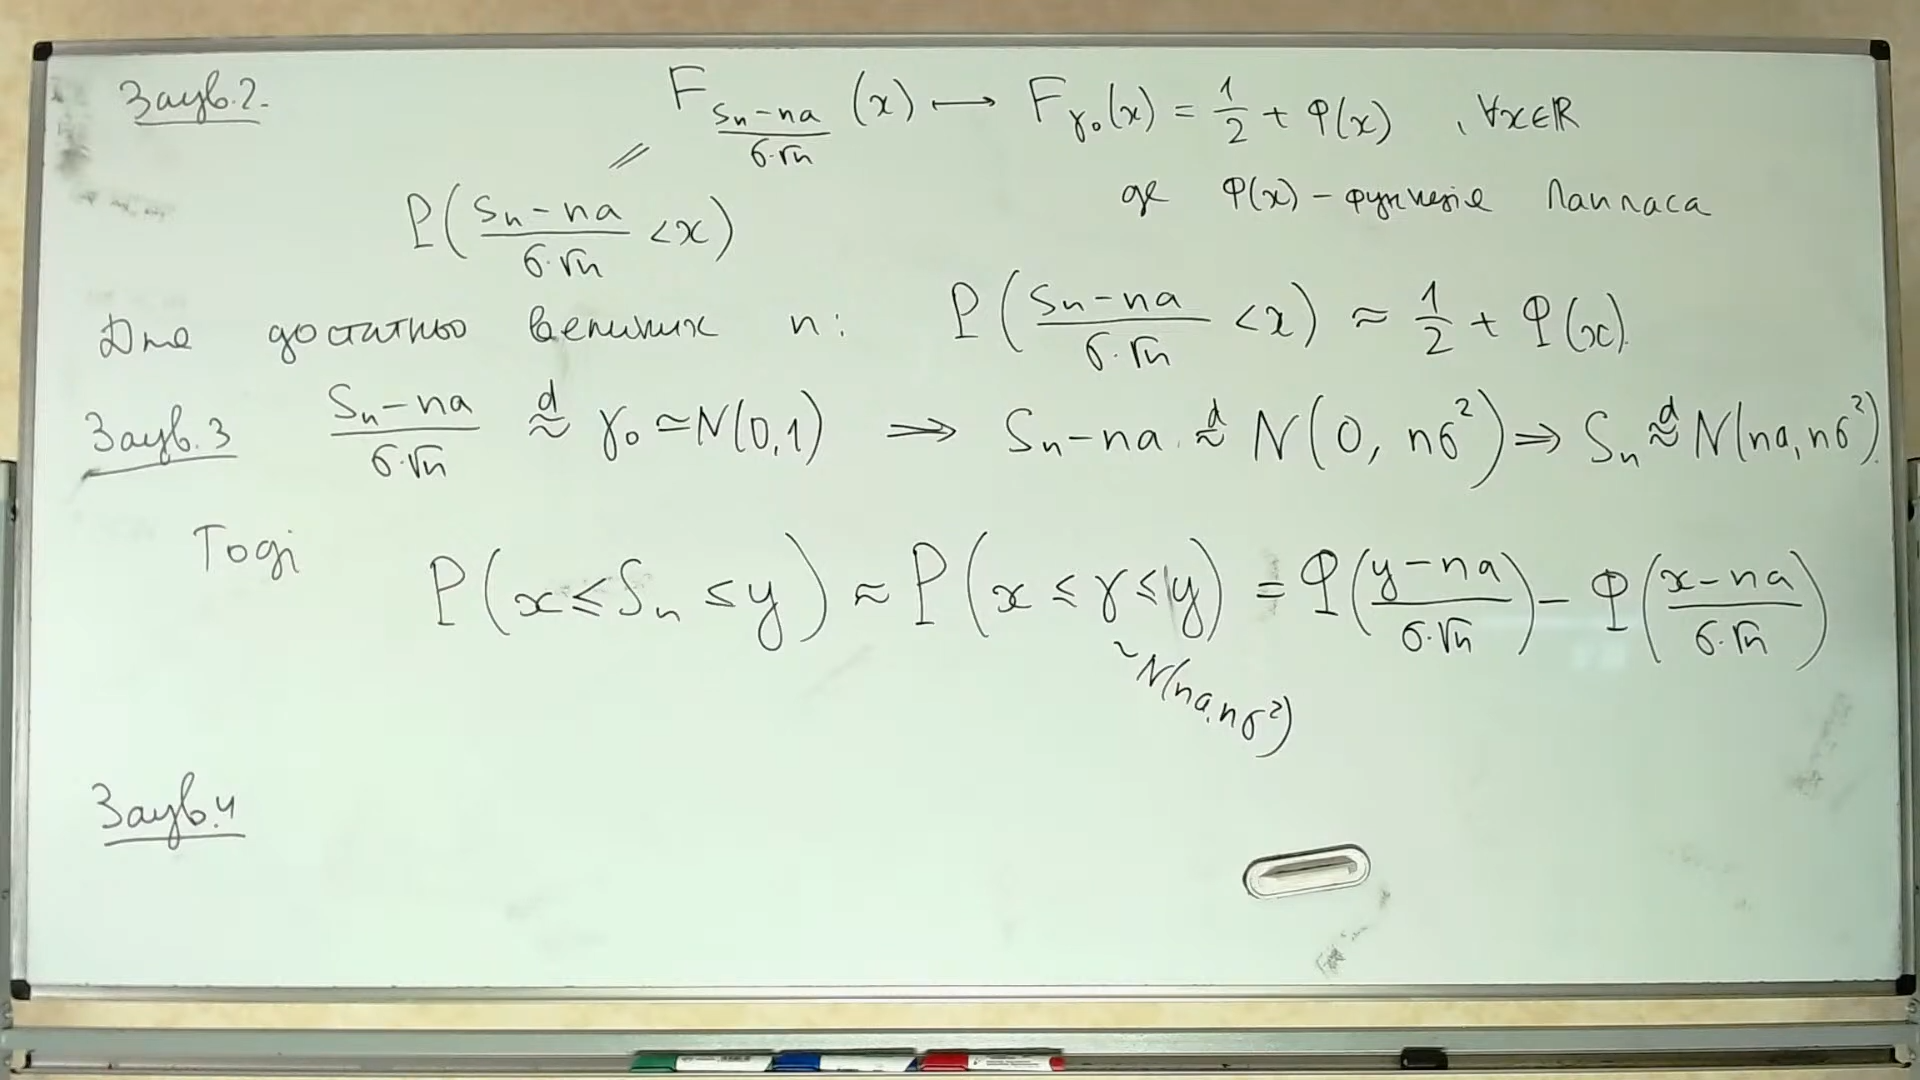
\includegraphics[width=0.5\textwidth]{images/bondarchuk_rgb}
  }\\
  \subfloat[Бінаризовані написи]{
    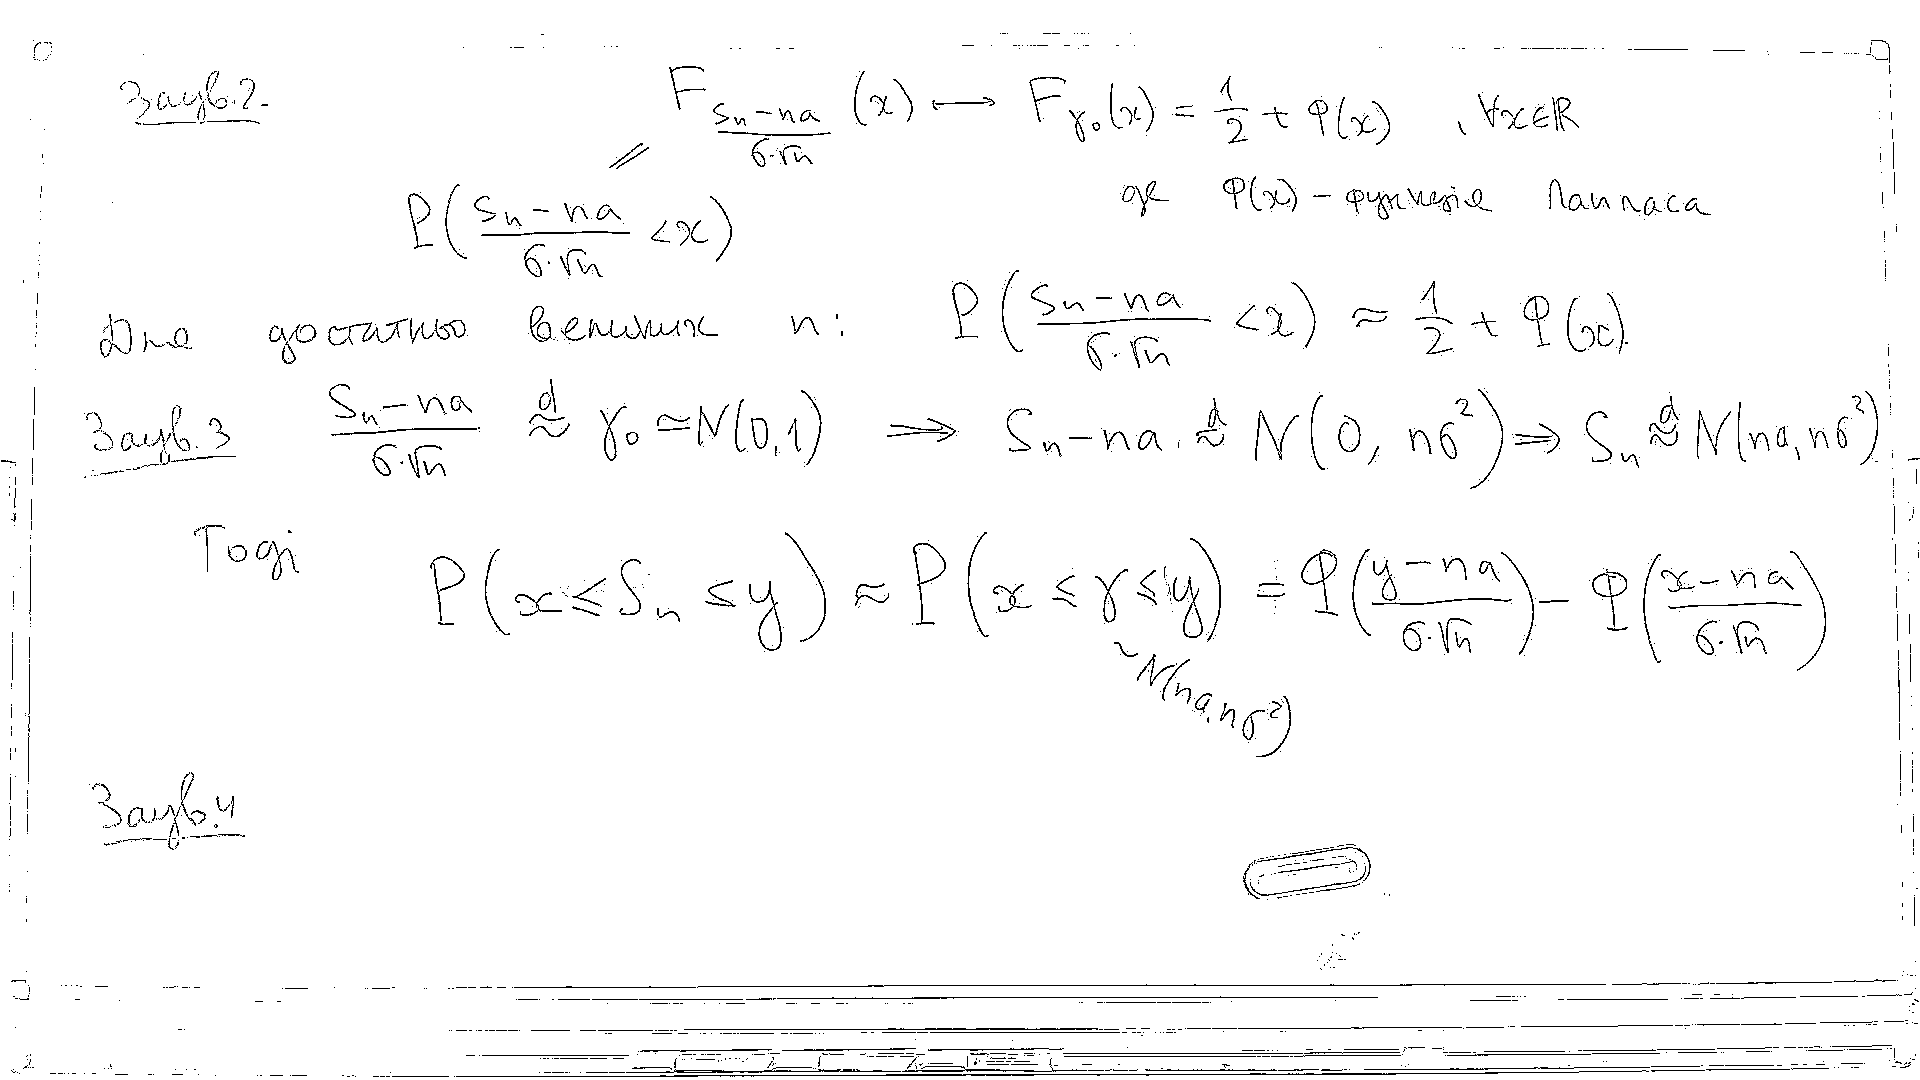
\includegraphics[width=0.5\textwidth]{images/bondarchuk_bin}
  }
  \caption{Приклад послідовного застосування оператору Лапласа та бінаризації Отсу
    з відео \cite{video:central_theorem}
    \label{fig:binarized_slide_example}
  }
\end{figure}
\begin{definition}
  Слайд ~---~ це та панорама \(W^{i}\), на якій відображено стан дошки
  напередодні стану з великою кількістю змін.
\end{definition}
Ми порівнюємо між собою не
кожну панораму, а пропускаємо вказану користувачем кількість \(q\)
панорам. Оскільки розміри слайду \(W^{i}\) і панорами
\(W^{i + s \cdot q}\) можуть бути різними, треба враховувати це у
процесі їх порівняння. Для цього розраховуємо горизонтальний зсув
$$x_{\min}^{'i} = \sum_{j = 1}^{q}{\min\left( x_{\min}^{i + s \cdot j},0 \right)}$$
і вертикальний зсув
$$y_{\min}^{'i} = \sum_{j = 1}^{q}{\min\left( y_{\min}^{i + s \cdot j},0 \right)}.$$
Користувач вказує кількість змін \(t \in \lbrack 0;1\rbrack\) між
слайдом та панорамою, яка є вирішальною для прийняття рішення щодо
створення нового слайду. Нехай \(L^{i}\) та \(L^{i + s \cdot q}\)~---~
панорами, отримані в результаті обробки оператором Лапласа панорам \(W^{i}\) та
\(W^{i + s \cdot q}\) відповідно. Якщо виконується нерівність
\begin{equation*}
  \sum_{(x,y) \in P^{i}}^{}| L^{i}(x,y) - L^{i + s \cdot q}( x - x_{\min}^{'i},y - y_{\min}^{'i} ) | > t \cdot | P^{i + s \cdot q} |,
\end{equation*}
бінаризовану \(W^{i}\) додаємо до списку слайдів, а в іншому випадку переходимо до
перевірки слайду \(W^{i + s \cdot q}\).